\documentclass{ctexart}
\usepackage[a4paper,top=2cm,bottom=2cm,left=3cm,right=3cm,marginparwidth=1.75cm]{geometry}
\usepackage{extarrows}
\usepackage{amssymb}

\usepackage{amsmath}
\usepackage{graphicx}
\usepackage[colorlinks=true, allcolors=blue]{hyperref}
\usepackage{CJKutf8}
\usepackage{CJKpunct}

\title{空间向量与立体几何}
\author{笙}

\begin{document}
\tableofcontents
\maketitle


\begin{abstract}
数学.选修一.第一章.
\end{abstract}

\section{空间向量及其运算}

\subsection{空间向量}

\subsubsection{定义}

空间向量：空间中，具有\textbf{大小和方向}的量。

模：空间向量的大小、

表示方法：有向线段；用字母\textbf{$a$,$b$}表示。

\subsubsection{特殊向量}

零向量：方向具有任意性，与任意向量均平行。

单位向量：模长为$1$的向量。

相等向量：方向相同且模相等。

相反向量：与\textbf{$a$}长度相等方向相反的量，记作\textbf{$-a$}。

方向向量：与\textbf{$a$}平行的非零向量。

\subsection{空间向量的线性运算}

即：平行四边形法则。

\subsection{共线向量与共面向量}

\subsubsection{共线向量}

共线向量：表示若干空间向量的有向线段所在直线\textbf{互相平行或重合}，则这些向量是共线向量。

共线向量基本定理：对任意向量\textbf{$a$}、\textbf{$b$}，有$a\parallel b\Longleftrightarrow a=\lambda b$

\subsubsection{共面向量}

共面向量：平行于同一平面的向量。

共面向量定理：若两向量\textbf{$a$}、\textbf{$b$}不共线，则向量\textbf{$p$}与向量\textbf{$a$}、\textbf{$b$}共面的充要条件是\textbf{存在唯一的有序实数对$(x,y)$}，\textbf{使得$p=xa+yb$}。

\subsubsection{应用}

$O$为空间内任意一点，点$A,B,P$三点共线的充要条件为：

\begin{equation*}
    \centering
    \overrightarrow{OP}=x\overrightarrow{OA}+y\overrightarrow{OB},x+y=1
\end{equation*}

$O$为空间内任意一点，点$A,B,C,P$四点共面的充要条件为：

\begin{equation*}
    \centering
    \overrightarrow{OP}=x\overrightarrow{OA}+y\overrightarrow{OB}+z\overrightarrow{OC},x+y+z=1
\end{equation*}

\subsection{空间向量的数量积}

\subsubsection{夹角}

范围：$0\leq \langle a,b\rangle \leq \pi$。

夹角为$0^{\circ}$时，两向量共线；夹角为$90^{\circ}$时，两向量垂直。

\subsubsection{数量积}

定义：$\left|a\right|\left|b\right|\cos\langle a,b\rangle$定义为数量积。

\begin{equation*}
    \centering
    a\cdot b=\left|a\right|\left|b\right|\cos\langle a,b\rangle
\end{equation*}

性质：

1.向量与自身的数量积是模的平方。

2.$a\cdot b=0\Longleftrightarrow a \perp b$(\textbf{$a$}、\textbf{$b$}为非零向量)。

3.夹角的计算。

4.对于任意向量\textbf{$a$}、\textbf{$b$}，总有$\left|a\cdot b\right|\leq\left|a\right|\left|b\right|$，当且仅当$a\parallel b$时等号成立。

\newpage

\subsubsection{投影向量}

作向量\textbf{$a$}在向量\textbf{$b$}上的投影向量：

先将它们平移到同一个平面$\alpha$内，利用平面上向量的投影得到与向量\textbf{$b$}共线的向量\textbf{$c$}，有

\begin{equation*}
    \centering
    c=\left|a\right|\cos\langle a,b\rangle \frac{b}{\left|b\right|}
\end{equation*}

此时称向量\textbf{$c$}为\textbf{$a$}在向量\textbf{$b$}上的投影。

\begin{figure}[h]
\centering
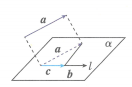
\includegraphics[width=0.2\linewidth]{Pic1.png}
\end{figure}

\bigskip

作向量\textbf{$a$}在平面$\alpha$上的投影向量：

分别由向量\textbf{$a$}的起点$A$和终点$B$作平面$\alpha$的垂线与垂足，得到向量$\overrightarrow{A'B'}$，其即为投影向量。

向量\textbf{$a$}与向量$\overrightarrow{A'B'}$的夹角即为向量\textbf{$a$}和平面$\alpha$的夹角。

\begin{figure}[h]
\centering
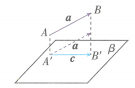
\includegraphics[width=0.2\linewidth]{Pic2.png}
\end{figure}

\newpage

\subsection{课后习题}

\begin{figure}[h]
\centering
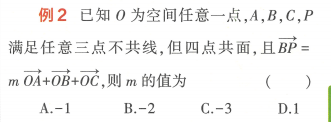
\includegraphics[width=0.6\linewidth]{Q1.png}
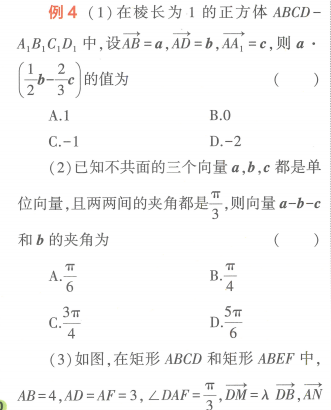
\includegraphics[width=0.6\linewidth]{Q2-1.png}
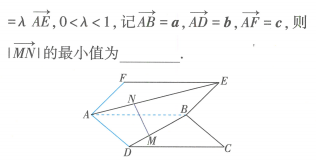
\includegraphics[width=0.6\linewidth]{Q2-2.png}
\end{figure}

\newpage

\section{平面向量基本定理}

\subsection{空间向量基本定理}

\subsubsection{定义}

若空间中存在三个不共面向量$a,b,c$，那么对任意一个空间向量$p$，\textbf{存在唯一的有序实数组$(x,y,z)$}，使得\textbf{$p=xa+yb+zc$}。

\subsubsection{基底与基向量}

基于上述定理，所有空间中的向量$p$组成的集合就是$\{p\| p=xa+yb+zc,x,y,z\in R\}$，这个集合可以看作由向量$a,b,c$生成的，我们把$\{a,b,c\}$叫做空间的一个\textbf{基底}，$a,b,c$叫做\textbf{基向量}。

\subsection{单位正交基底与空间向量的正交分解}

单位正交基地：空间的一个基底中的三个基向量两两垂直且均为单位向量，常用$\{i,j,k\}$表示。

对空间中的任意向量$p$，均可分解为三个向量$xi,yj,zk$，使得$p=xi+yj+zk$。

\newpage

\subsection{课后习题}

\begin{figure}[h]
\centering
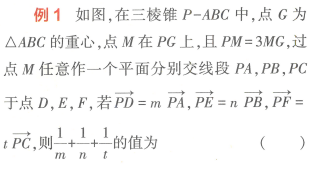
\includegraphics[width=0.6\linewidth]{Q3-1.png}
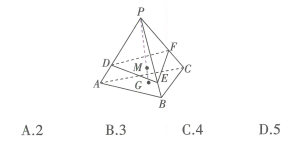
\includegraphics[width=0.6\linewidth]{Q3-2.png}
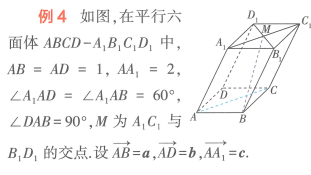
\includegraphics[width=0.6\linewidth]{Q4-1.png}
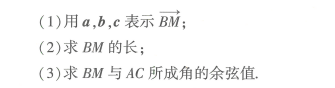
\includegraphics[width=0.6\linewidth]{Q4-2.png}
\end{figure}

\newpage

\section{空间向量及其运算的坐标表示}

\subsection{空间直角坐标系}

在空间中选定一点$O$，和一个单位正交基底$\{i,j,k\}$，以$O$为原点，分别以$i,j,k$的方向为正方向，以$i,j,k$的长度为单位长度，建立空间直角坐标系$Oxyz$。

\begin{figure}[h]
\centering
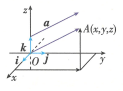
\includegraphics[width=0.3\linewidth]{Pic3.png}
\end{figure}

\subsection{空间向量的坐标表示}

设$A$为空间内任一点，$\overrightarrow{OA}=xi+yj+zk$，则称$(x,y,z)$为点$A$的坐标。

\subsection{空间向量运算的坐标表示}

对$Oxyz$空间内两点$A(x_1,y_1,z_1),B(x_2,y_2,z_2)$，有：

\begin{equation*}
    \centering
    \overrightarrow{AB}=\overrightarrow{OB}-\overrightarrow{OA}=(x_2-x_1,y_2-y_1,z_2-z_1)
\end{equation*}

对两向量$a(x_1,y_1,z_1),b(x_2,y_2,z_2)$，其运算有：

\begin{table}[h]
    \centering
    \begin{tabular}{c|c}
        \hline
        向量的和 & $a+b=(x_1+x_2,y_1+y_2,z_1+z_2)$ \\
        \hline
        向量的差 & $a-b=(x_1-x_2,y_1-y_2,z_1-z_2)$ \\
        \hline
        数乘 & $\lambda a=(\lambda x_1,\lambda y_1,\lambda z_1)$\\
        \hline
        数量积 & $a\cdot b=x_1x_2+y_1y_2+z_1z_2$\\
        \hline
    \end{tabular}
\end{table}

\subsection{空间向量平行与垂直的坐标表示}

对两向量$a(x_1,y_1,z_1),b(x_2,y_2,z_2)$。

当$b\neq 0$时，$a\parallel b\Longleftrightarrow a=\lambda b,(\lambda\in R)$。

$a\perp b\Longleftrightarrow a\cdot b=0$。

\subsection{公式}

\subsubsection{夹角公式}

两非零向量$a(x_1,y_1,z_1),b(x_2,y_2,z_2)$，有：

\begin{equation}
    \centering
    \cos\langle a,b\rangle=\frac{x_1x_2+y_1y_2+z_1z_2}{\sqrt{x_1^2+y_1^2+z_1^2}\cdot\sqrt{x_2^2+y_2^2+z_2^2}}
\end{equation}

\subsubsection{距离公式}

空间直角坐标系内两点$A(x_1,y_1,z_1),B(x_2,y_2,z_2)$，其两点间距离为：

\begin{equation}
    \centering
    \left|AB\right|=\sqrt{(x_2-x_1)^2+(y_2-y_1)^2+(z_2-z_1)^2}
\end{equation}

\subsubsection{定比分点坐标公式}

空间直角坐标系内两点$A(x_1,y_1,z_1),B(x_2,y_2,z_2)$，若点$M$满足$\overrightarrow{AM}=\lambda\overrightarrow{MB}(\lambda\in R,\lambda\neq -1)$，则点$M$的坐标为：

\begin{equation}
    \centering
    M(\frac{x_1+\lambda x_2}{1+\lambda},\frac{y_1+\lambda y_2}{1+\lambda},\frac{z_1+\lambda z_2}{1+\lambda})
\end{equation}

\subsubsection{三角形重心坐标公式}

对三角形$ABC$，其顶点坐标分别为$A(x_1,y_1,z_1),B(x_2,y_2,z_2),C(x_3,y_3,z_3)$，则其重心坐标为：

\begin{equation}
    (\frac{x_1+x_2+x_3}{3},\frac{y_1+y_2+y_3}{3},\frac{z_1+z_2+z_3}{3})
\end{equation}

\newpage

\subsection{课后习题}

\begin{figure}[h]
\centering
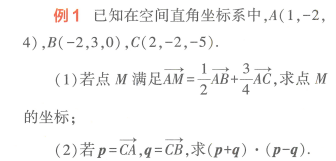
\includegraphics[width=0.6\linewidth]{Q5.png}
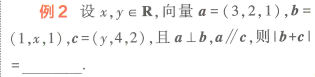
\includegraphics[width=0.6\linewidth]{Q6.png}
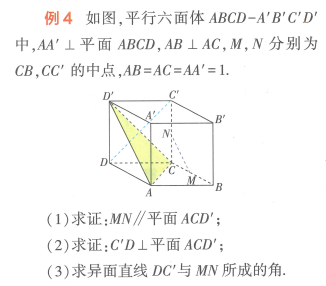
\includegraphics[width=0.6\linewidth]{Q7.png}
\end{figure}

\newpage

\section{空间向量的应用}

\subsection{空间中的向量表示}

\subsubsection{点的向量表示}

用$\overrightarrow{OP}$表示点$P$。

\subsubsection{直线的向量表示}

$\overrightarrow{OP}=\overrightarrow{OA}+ta=\overrightarrow{OA}+t\overrightarrow{AB}$。

\begin{figure}[h]
\centering
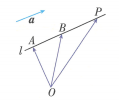
\includegraphics[width=0.3\linewidth]{Pic4.png}
\end{figure}

\subsubsection{平面的向量表示}

取定空间内一点$O$，空间内一点$P$位于平面$ABC$内的充要条件是，存在实数$x,y$，使得$\overrightarrow{OP}=\overrightarrow{OA}+x\overrightarrow{AB}+y\overrightarrow{AC}$。

\begin{figure}[h]
\centering
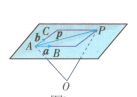
\includegraphics[width=0.3\linewidth]{Pic5.png}
\end{figure}

\subsection{平面的法向量}

\begin{figure}[h]
\centering
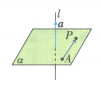
\includegraphics[width=0.3\linewidth]{Pic6.png}
\end{figure}

直线$l\perp \alpha$，取直线$l$的方向向量$a$，称其为平面$\alpha$的法向量。

给定一个点$A$和一个向量$a$，则过点$A$，且以$a$为法向量的平面唯一确定。

\newpage

\subsection{空间中线面位置关系的判定}

设直线$l,m$的方向向量分别为$a,b$，平面$\alpha,\beta$的法向量分别为$u,v$。

\begin{table}[h]
    \centering
    \begin{tabular}{c|c}
        \hline
        线线平行 & $l\parallel m\Longleftrightarrow a\parallel b\Longleftrightarrow \exists k\in R,s.t.a=kb$ \\
        \hline
        线面平行 & $l\parallel \alpha\Longleftrightarrow a\perp u\Longleftrightarrow a\cdot u=0$ \\
        \hline
        面面平行 & $\alpha\parallel\beta\Longleftrightarrow u\parallel v\Longleftrightarrow \exists k\in R,s.t.u=kv$ \\
        \hline
        线线垂直 & $l\perp m\Longleftrightarrow a\perp b\Longleftrightarrow a\cdot b=0$\\
        \hline
        线面垂直 & $l\perp \alpha\Longleftrightarrow a\parallel u\Longleftrightarrow\exists k\in R,s.t.a=ku$\\
        \hline
        面面垂直 & $\alpha\perp\beta\Longleftrightarrow u\perp v\Longleftrightarrow u\cdot v=0$\\
        \hline
    \end{tabular}
\end{table}

\subsection{计算空间距离}

\subsubsection{直线外一点到直线的距离}

\begin{figure}[h]
\centering
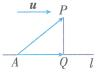
\includegraphics[width=0.3\linewidth]{Pic7.png}
\end{figure}

直线$l$的单位方向向量为$u$，$A$是直线$l$上的定点，$P$是直线$l$外一点。

设$\overrightarrow{AP}=a$，则向量$\overrightarrow{AP}$在直线$l$上的投影向量为，则：

\begin{equation*}
    \centering
    \overrightarrow{AQ}=(a\cdot u)u
\end{equation*}

\begin{equation*}
    \centering
    PQ=\sqrt{\left|\overrightarrow{AP}\right|^2-\left|\overrightarrow{AQ}\right|^2}=\sqrt{a^2-(a\cdot u)^2}
\end{equation*}

\subsubsection{平面外一点到平面的距离}

\begin{figure}[h]
\centering
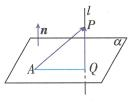
\includegraphics[width=0.3\linewidth]{Pic8.png}
\end{figure}

平面$\alpha$的法向量为$n$，$A$是平面$\alpha$内的定点，$P$是平面$\alpha$外一点，过点$P$作平面$\alpha$的垂线$l$，交平面$\alpha$于点$Q$，则$n$是直线$l$的方向向量，点$P$到平面$\alpha$的距离就是$\overrightarrow{AP}$在直线$l$上的投影向量$\overrightarrow{QP}$的长度。

\begin{equation*}
    \centering
    PQ=\left|\overrightarrow{AP}\cdot\frac{n}{\left|n\right|}\right|=\left|\frac{\overrightarrow{AP}\cdot n}{\left|n\right|}\right|=\frac{\left|\overrightarrow{AP}\cdot n\right|}{\left|n\right|}
\end{equation*}

\subsubsection{两平面之间的距离}

转化为点到平面的距离求解。

\subsection{计算空间角}

\subsubsection{异面直线夹角}

异面直线$l_1,l_2$的夹角为$\theta$，方向向量分别为$u,v$，则：

\begin{equation*}
    \centering
    \cos\theta=\left|\cos\langle u,v\rangle\right|=\left|\frac{u\cdot v}{\left|u\right|\left|v\right|}\right|=\frac{\left|u\cdot v\right|}{\left|u\right|\left|v\right|}
\end{equation*}

\subsubsection{直线与平面所成的角}

\begin{figure}[h]
\centering
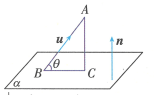
\includegraphics[width=0.3\linewidth]{Pic9.png}
\end{figure}

直线$AB$与平面$\alpha$相交于$B$，设直线$AB$与平面$\alpha$所成的角为$\theta$，直线$AB$的方向向量为$u$，平面$\alpha$的法向量为$n$，则：

\begin{equation*}
    \centering
    \sin\theta=\left|\cos\langle u,n\rangle\right|=\left|\frac{u\cdot n}{\left|u\right|\left|n\right|}\right|=\frac{\left|u\cdot n\right|}{\left|u\right|\left|n\right|}
\end{equation*}

\subsubsection{平面与平面的夹角}

\begin{figure}[h]
\centering
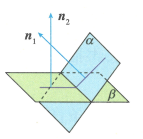
\includegraphics[width=0.3\linewidth]{Pic10.png}
\end{figure}

平面$\alpha$与平面$\beta$相交，形成四个二面角，其中不大于$90^{\circ}$的角称为两平面的夹角。

设平面$\alpha,\beta$的法向量分别是$n_1,n_2$，夹角为$\theta$，则：

\begin{equation*}
    \centering
    \cos\theta=\left|\cos\langle n_1,n_2\rangle\right|=\left|\frac{n_1\cdot n_2}{\left|n_1\right|\left|n_2\right|}\right|=\frac{\left|n_1\cdot n_2\right|}{\left|n_1\right|\left|n_2\right|}
\end{equation*}

\newpage

\subsection{课后习题}

\begin{figure}[h]
\centering
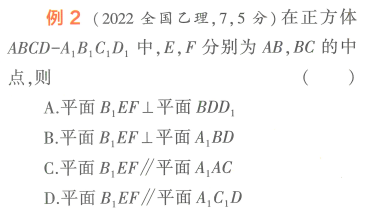
\includegraphics[width=0.5\linewidth]{Q8.png}
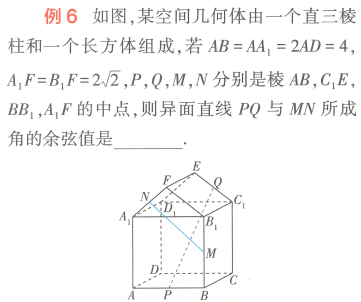
\includegraphics[width=0.5\linewidth]{Q9.png}
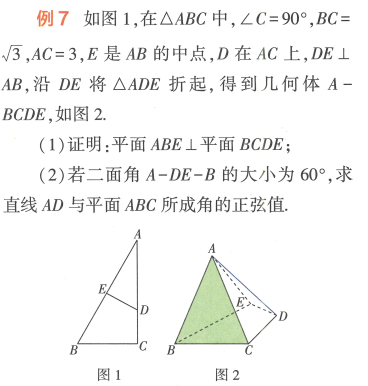
\includegraphics[width=0.5\linewidth]{Q10.png}
\end{figure}

\begin{figure}[p]
\centering
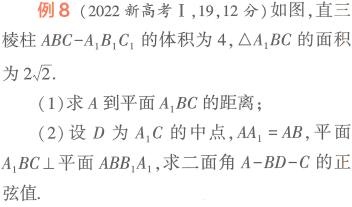
\includegraphics[width=0.7\linewidth]{Q11-1.png}
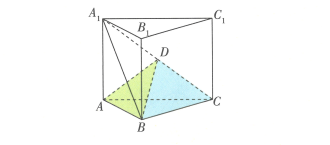
\includegraphics[width=0.7\linewidth]{Q11-2.png}
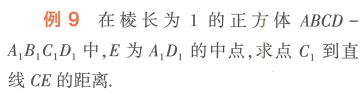
\includegraphics[width=0.7\linewidth]{Q12.png}
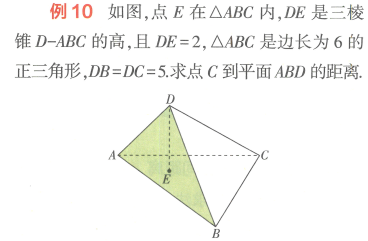
\includegraphics[width=0.7\linewidth]{Q13.png}
\end{figure}

\begin{figure}[p]
\centering
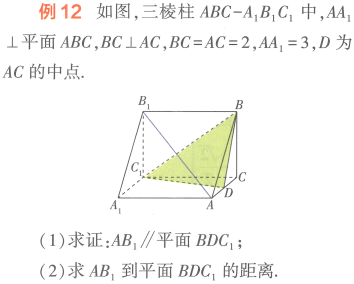
\includegraphics[width=0.7\linewidth]{Q14.png}
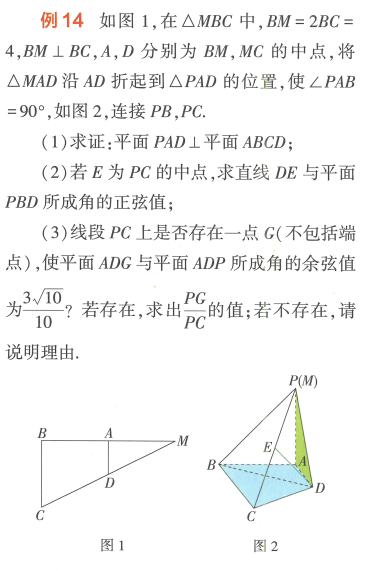
\includegraphics[width=0.7\linewidth]{Q15.png}
\end{figure}

\begin{figure}[p]
\centering
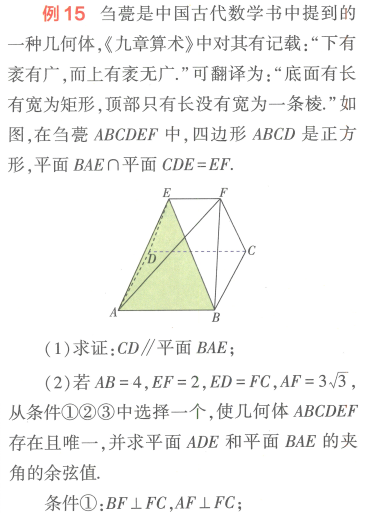
\includegraphics[width=0.7\linewidth]{Q16-1.png}
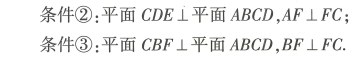
\includegraphics[width=0.7\linewidth]{Q16-2.png}
\end{figure}

\end{document}